\documentclass{beamer}

\mode<presentation> {
\usetheme{default}
\usecolortheme{dolphin}
}

\usepackage{graphicx}
\usepackage{booktabs}
\usepackage{amsthm}
\usepackage{subfigure}
\usepackage{bbm}
\usepackage{tikz}
\usetikzlibrary{shapes,automata}

\newcommand{\iter}[2]{#1^{(#2)}}
\newcommand{\transpose}[1]{#1^{\mathsf{T}}}
\newcommand{\iter}[2]{#1^{(#2)}}
\newcommand{\parens}[1]{ \left( #1 \right) }
\newcommand{\prob}{\mathbb{P}}

\title[Short title]{Exploring PageRank} 
\author{Nathanael Gentry}
\institute[LU]{MATH 321}
\date{24 April 2019}

\begin{document}
\begin{frame}
\titlepage
\end{frame}

\section{First Steps}
\begin{frame}[label=web]{A Miniscule Web}
    	\begin{figure}[h]
		\centering \scalebox{0.75}{\begin{tikzpicture}[
			scale=0.6,
            > = stealth,
			shorten > = 1pt,
			auto,
			node distance = 3cm,
			semithick]
			\tikzstyle{every state}=[
			draw = black,
			thick,
			fill = white,
			minimum size = 4mm]
		
			\node[state] (a) {$p_1$};
			\node[state] (b) [above right of=a] {$p_2$};
			\node[state] (c) [right of=a] {$p_3$};
			\node[state] (d) [below right of=a] {$p_4$};
			\node[state] (e) [right of=c] {$p_5$};
		
			\path[->] (a) edge node {} (b);
			\path[->] (a) edge node {} (d);
			\path[->] (a) edge node {} (c);
			\path[->] (c) edge node {} (b);
			\path[->] (d) edge node {} (c);
			\path[->] (e) edge node {} (b);
			\path[->] (b) edge [bend left=45] node {} (e);
			\path[->] (d) edge node {} (b);
			\path[->] (e) edge node {} (c);
			\path[->] (d) edge node {} (e);
		\end{tikzpicture}}
		\caption{A Miniscule Web}
		\label{fig:web}
	\end{figure}
\end{frame}

\begin{frame}{Intuition}
    We view a hyperlink to a page as an endorsement of importance from the linking page.\\
    \vspace{1mm}
    If a page is not very selective of its endorsements, its endorsements should be less prestigious than those given by a more discriminating page.
\end{frame}

\begin{frame}{Intuition}
    Let $N^-_i$ represent the set of $p_i$'s predecessors, and let $N^+_i$ represent the set of $p_i$'s successors, and note that $|N^+_i|$ gives the out-degree of $p_i$. We thus define the importance score $\pi_i$ of a page $p_i$:
 	\begin{equation*}
 		\pi_i = \sum_{p_j\in N^-_i}{\frac{\pi_j}{|N^+_i|}}.
 	\end{equation*}
\end{frame}

\begin{frame}{Iteration}
     Take some initial score vector $\iter{\pi}{0}$, say a uniform distribution $\pi = [1/|\mathcal{W}|]$. Then, we define an iterative calculation for an iterator $t\geq 1$ to refine the initial distribution:
 	 \begin{equation*}
	 	\iter{\pi}{t+1}_i = \sum_{p_j\in N^-_i}{\frac{\iter{\pi}{t}_j}{|N^+_i|}}.
 	\end{equation*}
\end{frame}

\begin{frame}{Hyperlink Matrix}
     We encode the system given by the previous equation over $\mathcal{W}$ in a hyperlink matrix:
 	\begin{equation*}
 		H_{ij}=\begin{cases}
 			1/|N^+_i|, & \text{if } p_i \in N^-_j; \\
 			0, & \text{otherwise}.
 		\end{cases}
 	\end{equation*}
\end{frame}

\againframe{web}

\begin{frame}{A Simple Example}
    \begin{figure}[t!]
        \centering
        \begin{subfigure}
            \centering
            $\begin{bmatrix}
                0 & 1/3 & 1/3 & 1/3 & 0 \\
                0 & 0 & 0 & 0 & 1 \\
                0 & 1 & 0 & 0 & 0 \\
                0 & 1/3 & 1/3 & 0 & 1/3 \\
                0 & 1/2 & 1/2 & 0 & 0
            \end{bmatrix}$
            \caption{Hyperlink Matrix for Figure \ref{fig:web}}
        \end{subfigure}
        \vspace{1em}
        \begin{subfigure}
        \centering
        \begin{tabular}{|c||c|c|c|c|c|}
             \hline
             $k$ & $\iter{\pi_1}{k}$ & $\iter{\pi_2}{k}$ & $\iter{\pi_3}{k}$ & $\iter{\pi_4}{k}$ & $\iter{\pi_5}{k}$ \\
             \hline\hline
             0 & 0.2 & 0.2 & 0.2 & 0.2 & 0.2 \\
             1 & 0 & 0.433 & 0.233 & 0.067 & 0.267 \\
             2 & 0 & 0.389 & 0.156 & 0 & 0.456 \\
             3 & 0 & 0.383 & 0.228 & 0 & 0.390 \\
             4 & 0 & 0.422 & 0.194 & 0 & 0.383 \\
             \hline
        \end{tabular}
        \caption{Score Iteration for Figure \ref{fig:web}}
        \end{subfigure}
        
        \label{fig:iterative_example}
    \end{figure}
\end{frame}

\section{Markov Chains}
\subsection{Stochasticity}
\begin{frame}{Stochasticity}
    Consider a vector $d$, where $d_i=1$ if page $p_i$ dangles and $d_i=0$ otherwise, and let $v$ be a distribution over all pages in $\mathcal{W}$, given as a row vector. We stochasticize $H$ thusly:
	\begin{equation*}
	    \label{eqn:S}
		S=H + d \transpose{v}.
	\end{equation*}
\end{frame}

\begin{frame}{Stochasticity}
	\begin{theorem}
	    All stochastic matrices $S$ have spectral radius $\rho(S)=1$, with an eigenvalue $\lambda = \rho(S)$ on the spectral circle.
	\end{theorem}
	\begin{proof}
	    Let $\mathbbm{1}$ represent a vector of ones. The row-stochasticity of $S$ implies $\Vert S \Vert_{\infty} = 1$, i.e., $S \mathbbm{1} = \mathbbm{1}$. Thus, $(1, \mathbbm{1})$ provides a right eigenpair for every stochastic matrix. Now, consider an eigenpair $(v, \lambda)$ of a stochastic matrix $S$ and suppose $|\lambda| > 1$. Then, the vector given by $|\lambda|^n v = S^n v$ grows exponentially, so at least one $(S^n)_{ij} > 1$ for some $n$. This, however, violates the stochasticity of $S$ and its powers. Thus, we conclude that $|\lambda| \leq 1$, and since we have already 1 as an eigenvalue, we conclude the spectral radius $\rho(S)=1$.
	\end{proof}
	
\end{frame}

\begin{frame}{Markov Property}
    A discrete-time stochastic process $\{X_t\}_{t \in T}$ for a countable set $T$ over a finite state space $\Omega = \{s_i\}_{i=0}^{n}$ is a Markov chain if the Markov property holds for each $t$:
	\begin{align*}
		\prob(X_{t+1} = s_j \mid &X_t = s_{i_t}, X_{t-1} = s_{i_{t-1}},\cdots, X_0 = s_{i_0}) \\ &= \prob(X_{t+1} = s_j \mid X_t=s_{i_{t}}).
	\end{align*}
	\vspace{2mm}
	\pause \centering \textit{Markov chains are memoryless.}
\end{frame}

\begin{frame}{Transition Probabilities}
    We encode the $k$-step transition probabilities for a homogeneous Markov chain in a stochastic matrix of dimension $|\Omega| \times |\Omega|$:
	\begin{equation*}
		\iter{P}{k} = [ \iter{p}{k}_{ij} ] = [ \prob(X_{t+k} = s_j \mid X_t = s_i) ] = [ \prob(X_{t} = s_j \mid X_0 = s_i) ].
	\end{equation*}
\end{frame}

\begin{frame}{Markovian Iteration}
    Consider a distribution $\iter{v}{\ell}$ over $\Omega$, defined by $\iter{v}{\ell}_i = \prob(X_\ell = i)$. Then, by the total law of probability, we calculate the following:
    \begin{align*}
        \iter{v}{\ell}_i &= \sum_{s_k\in\Omega}{\prob(X_0 = s_k) \prob(x_\ell = s_i \mid X_0 = s_k)} \\
        &= \sum_{k\leq |\Omega|}{\parens{\iter{v}{0}_k \iter{p}{\ell}_{ki}}}.
    \end{align*}\\
    \vspace{2mm}
    We conclude that $\iter{v}{\ell} = \iter{v}{0} \iter{P}{\ell} = \iter{v}{0} P^\ell$, for some initial distribution $\iter{v}{0}$.
\end{frame}

\subsection{Stationarity}
\begin{frame}{Stationary Distribution}
     We can take the stochastic process $\{X_t\}_{t \in T}$ underlying a Markov chain as a categorical distribution over $\mathcal{S}$, the state space. \\
     \vspace{2mm}
     By Brouwer's fixed point theorem, within this process must be a $P$-invariant distribution, i.e., an eigenvector of $P$. \\
     \vspace{2mm}
     We denote this fixed distribution $\pi$, given as a row vector, such that $\pi P = \pi$. That is, $\pi_i = \prob(X_t = s_i)$ for all $t$ over all states.
\end{frame}

\begin{frame}{Limiting Distribution}
    Consider a stationary distribution $\pi$ that is also a limiting distribution:
	\begin{equation*}
		\pi = \lim_{k\to\infty}{{\iter{\pi}{k}}} = \lim_{k\to\infty}{\parens{{\iter{\pi}{0}} P^k}}.
	\end{equation*}\\
	\vspace{2mm}
	\textit{Note}: In a Markov chain where the transition matrix converges, an almost-arbitrary initial distribution $\iter{\pi}{0}$ will eventually converge upon $\pi$.
\end{frame}T22tshow

\section{Perron-Frobenius Theory}
\begin{frame}{Irreducibility of Chains}
    In a Markov chain, states $s_i$ and $s_j$ communicate if $\iter{P}{k}_{ij} > 0$, for some iterator (nonnegative integer) $k$. That is, there is a random walk of nonzero probability between states $s_i$ and $s_j$. Communicativity is easily shown to be an equivalence relation.\\
    \vspace{2mm}
    A Markov chain is irreducible if it contains a single communicating class.
\end{frame}

\begin{frame}{Irreducibility of Graphs}
    Equivalently, a graph is irreducible if it has no strongly connected components smaller than itself. If a graph $\mathcal{G}$ is \textit{reducible}, we can permute its vertices to obtain a canonical form for the acjacency matrix $A$:
    \begin{equation*}
	    R = \transpose{P} A P = 
	    \begin{bmatrix}
		    X & Y \\
		    0 & Z
	    \end{bmatrix}.
	\end{equation*} \\
	\vspace{2mm}
	If $\iter{A}{k}_{ij} > 0$ for all distinct vertex pairs $(i,j)$ and $k = k_{(i,j)}$, then $\mathcal{G}$ is strongly connected and $A$ is therefore irreducible.
\end{frame}

\begin{frame}{Significance of Irreducibility}
    If the chain is reducible so not all pages communicate, then there is a nonzero probability that the random surfer ventures off and visits some pages only finitely many times. Thus, as time passes, the probability of visiting these pages drops to zero.
\end{frame}

\begin{frame}{Periodicity}
    We define the period of a state by $d(s_i)=\text{gcd}\{n\in \mathbb{Z}_{\geq 0} : \iter{p}{n}_{ii} > 0 \}$. In other words, a random walk from state $s_i$ can only return to $s_i$ in multiples of $d(s_i)$ steps. \\
    \begin{theorem}
        If Markov states $s_i$ and $s_j$ communicate, then $d(s_i) = d(s_j)$.
    \end{theorem}\\
    \vspace{2mm}
     When $P$ is irreducible, $d(P)$ is well-defined; every state has the same period. When $d(P) = 1$, the chain is aperiodic.
\end{frame}

\begin{frame}{Primitivity}
    \begin{lemma}
        For an irreducible aperiodic Markov chain with transition matrix $P$, there is some bound $t_i$ beyond which $\iter{p}{t}_{ii} > 0$ for all $t \geq t_i$ over all states.
    \end{lemma}
    
    \begin{theorem}
        For the chain considered above, there is a $t$ that gives $\iter{p}{t}_{ij} > 0$ over all states, and so $P^t > 0$.
    \end{theorem}\\
    \vspace{2mm}
    We take this result as the definition of matrix primitivity.
\end{frame}

\begin{frame}{Perron-Frobenius Theorem}
	If $A$ is a primitive matrix, then
	\begin{enumerate}
		\item The spectral radius $\rho(A)$ equals some real eigenvalue $\lambda_1$;
		\item This eigenvalue (the Perron root) is simple, and it is the only eigenvalue on the spectral circle;
		\item The Perron root has unique, strictly positive left and right eigenvectors (Perron vectors);
		\item These left and right Perron vectors are, up to normalization, the only nonnegative eigenvectors of $A$.
	\end{enumerate}
\end{frame}

\section{Limiting Distributions}
\begin{frame}{Matrix Limits}
    \begin{theorem}
       For a square real matrix $A$, we have $A^n \to 0$ as $n\to\infty$ if and only if $\rho(A) < 1$, and the limit does not exist when $\rho(A) > 1$.
    \end{theorem}
    
    \begin{theorem}
        For $A$ given ahove, when $\rho(A) = 1$ is a simple eigenvalue with respective left and right eigenvectors $x$ and $y$, the limit converges:
        \begin{equation*}
            \lim_{k\to\infty}{A^k} = \frac{x y^*}{x^* y},
        \end{equation*}
        where $\frac{x y^*}{x^* y}$ projects onto the eigenspace $\mathcal{E}_1$.
    \end{theorem}
\end{frame}

\begin{frame}{Limiting Distributions}
    All stochastic matrices have right eigenvector $\mathbbm{1}$, and a primitive matrix $P$ has left eigenvector $\pi$ (the stationary distribution). Thus, we have:
    \begin{align*}
        \lim_{k\to\infty}{{\iter{\pi}{k}}} &= \lim_{k\to\infty}{\parens{{\iter{\pi}{0}} P^k}} \\ &= \iter{\pi}{0} \parens{\frac{\mathbbm{1} \pi}{\pi \mathbbm{1}}} \\ &= \parens{\iter{\pi}{0} \mathbbm{1}} \pi \\ &= \pi. 
    \end{align*}
\end{frame}

\begin{frame}{Power Iteration}
    Suppose a square matrix $A$ has $n$ eigenpairs $\{ (\lambda_i,x_i)_{i\leq n} \}$ with $\lambda_1$ as a dominant eigenvalue.\\
    \vspace{2mm}
    Consider a starting vector $x^{(0)}=\sum_i{\gamma_i x_i}$ for scalars $\gamma_i$. Then, we again consider an iterative calculation:
	\begin{equation*}
		\iter{x}{k} = A^k \iter{x}{0} = \sum_{i=1}^{k}{\gamma_i \lambda_i^k x_i} = \lambda_1^k\parens{\gamma_1 x_1 + \sum_{i=2}^{k}{\gamma_i \frac{\lambda_i}{\lambda_1} x_i}} \to \lambda_1^k \gamma_1 x_1.
	\end{equation*}
	\pause Since $\lambda_i<\lambda_1$ for $i>1$, the sum approaches 0 as $k\to\infty$.
\end{frame}

\begin{frame}{The Web Graph [1]}
        \begin{figure}
        \centering
        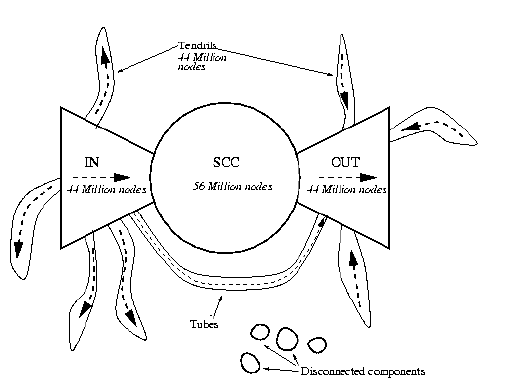
\includegraphics[scale=0.6]{../paper/images/bow-tie}
        \label{fig:bow-tie}
    \end{figure}
\end{frame}

\begin{frame}{Taming the Web}
    We interpreted the stochastic Web matrix $S$ as the matrix of probabilities that a random web surfer follows links from a page or chooses another randomly when it hits a dead end. However, \textit{human} Web surfers often get bored. They might suddenly elect to teleport -- shift course altogether and visit a random page.\\
    \vspace{2mm}
    \pause Consider a distribution $u$ over all Web pages. We model this teleportation behavior with a rank-one matrix $T = \mathbbm{1} \cdot \transpose{u}$.
\end{frame}

\begin{frame}{The Google Matrix}
    Now, consider a matrix $G$ formed from a convex combination of $S$ and $T$:
	\begin{equation*}
	    \label{google_matrix}
		G = \alpha S + (1-\alpha)T.
	\end{equation*}
	
	\pause Every page has some connection of nonzero probability to every other page, and our process is still stochastic. The teleportation adjustment thus provides primitivity and guarantees a limiting distribution, from which we can rank pages.
\end{frame}

\begin{frame}{Convergence Speed}
    The speed of convergence depends upon how quickly $\parens{\frac{\lambda_i}{\lambda_1}}^k \to 0$. Unfortunately, due to its \textit{scale-free} nature, the raw Web graph as $\lambda_2$ (a subdominant eigenvalue) close to 1. \\
    \vspace{2mm}
    \pause Even with the primitivity adjustment, the Web graph is only weakly irreducible. \\
    \vspace{2mm}
    \pause Choosing $\alpha \approx 0.85$ has been empirically shown to balance fidelity with efficiency.
\end{frame}

\begin{frame}{Further Investigations}
    \begin{enumerate}
        \item What about link spammers -- those who try to trick PageRank by manipulating the link structure of the Web?
        \item How sensitive is the calculation to the always-changing Internet?
        \item How can we coax the iterative calculation to converge more quickly? 
    \end{enumerate}
\end{frame}

\begin{frame}[allowframebreaks]
        \frametitle{References}
        \bibliographystyle{amsalpha}
        \bibliography{../references.bib}
\end{frame}
\end{document}